\newpage
\section{Dynamic network analysis}

  \subsection{Discretisation of data}
  
    Because the messages are posted on this forum virtually every minute the information about them might be considered as being continuous in time. In order to study the evolution of the network in time, there is a need to define discrete time intervals that will split the network in parts. Networks that are dynamic are called longitudinal networks.
    \\\\
    The time interval using which the data had to be split had to be determined empirically with a network to be kept in a size that would be representational. The choice was between a \emph{week-long}, \emph{two weeks}-long and a \emph{month}-long interval. Eventually, a \emph{$30$ day}-long time interval was selected, main reason being the fact that the date span of downloaded messages was almost 12 years long which created 141 data buckets. Additionally, message threads are often more than a week long, so we did want to avoid the situation where most threads are split into several buckets. It also allowed different kind of distributions stand out more because they were created with more data.
    
    The biggest downside was that the network sizes were still very big, thus all computations that had to be performed on a whole network took more time.
    
  \subsection{Estimating users' opinions about products} \label{sec:opinion_estimation}
  
    In order to estimate the opinions different users have about different products I had to prepare a script traversing the posts saved in my database and saving a value representing opinion. I had to create a separate table in my database for that, which structure is shown in table \ref{tab:db_opinions}.
    \begin{table}[H]
      \begin{tabularx}{\textwidth}{|L{0.3}|L{1.7}|} \hline
        \rowcolor[gray]{0.75} \textbf{Field} & \textbf{Description} \\\hline
        user\_id & Unique user reference; found in users table as id. \\
        word\_id & Unique word reference; found in words table as id. \\
        opinion & A real value representing opinion. \\
        bucket & Bucket number from which the opinion value was calculated. \\\hline
      \end{tabularx}
      \caption{Opinions table structure.}
      \label{tab:db_opinions}
    \end{table}

    The script was based on algorithm \ref{alg:estimate_user_keyword}. I have run it against every bucket, first gathering the list of users and keywords in that bucket.
    The algorithm was ran for every user and keyword. It fetched all messages written by the user in a bucket it was ran for. Then for every post it has checked whether the keyword was used within the post and returned position of each occurrence of that word. The position was established to be the $n$th \textquote{token} in the message, where \textquote{tokens} were obtained in the exact same way as words in section \ref{sec:text_segmentation}. Then the algorithm extracted all words marked as opinions from the message body and for each of these opinions it has checked their position as it did with keywords. Next, it has checked whether the opinion was \emph{positive} or \emph{negative} and applied a measure on a keyword based on squared distance between itself and the opinion biased positively or negatively.
    \begin{algorithm}[H]
      \begin{algorithmic}[1]
        \Procedure{EstimateOpinion}{user, keyword, bucket}
          \State estimate $\gets 0$
          \State posts $\gets$ \textsc{Posts}(user, bucket)
          \ForAll{post \textbf{in} posts} 
            \State keywordPositions $\gets$ \textsc{KeywordPositions}(keyword, post)
            \ForAll{keywordPosition \textbf{in} keywordPositions}
              \State opinions $\gets$ \textsc{Opinions}(post)
              \ForAll{opinion \textbf{in} opinions}
                \State opinionSign $\gets$ \textsc{OpinionSign}(opinion)
                \State opinionPosition $\gets$ \textsc{OpinionPosition}(opinion, post)
                \State distance $\gets$ |keywordPosition - opinionPosition|
                \State estimate $\gets$ estimate + (opinionSign / distance$^2$)
              \EndFor
            \EndFor
          \EndFor
          \State \textbf{return} estimate
        \EndProcedure
      \end{algorithmic}
      \caption{Estimating user's opinion about product.}
      \label{alg:estimate_user_keyword}
    \end{algorithm}

    \subsubsection{Measure}

      Let $e_o$ be an opinion estimate obtained using a method described above. Its value should be found in a range described by the following sum
      \begin{equation}
        \frac{1}{1^2} + \frac{1}{2^2} + \frac{1}{3^2} + \frac{1}{4^2} + \ldots = \sum_{n=1}^{\infty} \frac{1}{n^2} = \frac{\pi^2}{6} \mbox{,} \label{eqn:estimate}
      \end{equation}
      and as each keyword can have opinions written before and after itself, we have two multiply the sum in equation \ref{eqn:estimate} by a factor of $2$. Hence,
      \begin{equation}
        -\frac{\pi^2}{3} \leq e_o \leq \frac{\pi^2}{3} \mbox{.} \label{eqn:estimate_limits}
      \end{equation}
      
      Application of squared distance as a base for the measure favours opinions that are very close to keywords. This was extremely important especially for long posts so that keywords mentioned at the end of the message did not get influenced by an opinion mentioned at the beginning of it. With this approach it is expected for the most opinions to be found in a range of $[\sfrac{1}{4};\sfrac{1}{4}]$---most opinions would be generally no further away than 2 words from a keyword.
      
      Because measuring data in such way is not perfect and may create results contradictory to the real data I have decided to introduce a \emph{neutral} opinion using the middle range of the numbers. Hence, opinions were assigned in a following way:
      \begin{itemize}
        \item \emph{positive:} $L \leq e_o \leq \frac{\pi^2}{3}$,
        \item \emph{neutral:} $-L < e_o < L$,
        \item \emph{negative:} $-\frac{\pi^2}{3} \leq e_o \leq L$,
      \end{itemize}
      where $L = 0.01$ is an empirically found constant allowing for fairly even division of opinion types. Table \ref{tab:opinion_number} shows the number of opinions found, divided by the type of the opinion.
      \begin{table}[H]
        \centering
        \begin{tabularx}{\textwidth}{|L{1}|L{1}|L{1}|L{1}|} \hline
          \rowcolor[gray]{0.8} \textbf{Positive} & \textbf{Neutral} & \textbf{Negative} & \textbf{Total} \\\hline
          $4,219,548\;(42.99\%)$ & $3,398,282\;(34.62\%)$ & $2,197,055\;(22.39\%)$ & $9,814,885\;(100\%)$ \\\hline
        \end{tabularx}
        \caption{Number of opinions about products found, by the opinion type.}
        \label{tab:opinion_number}
      \end{table}

      \begin{figure}[H]
        \centering
        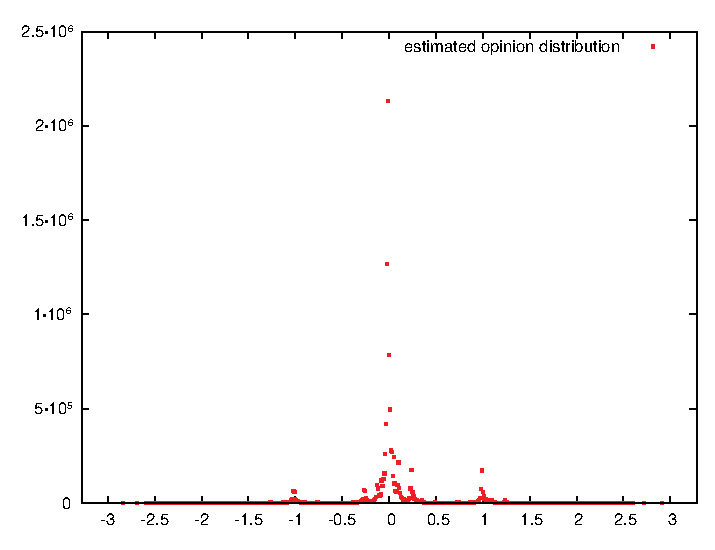
\includegraphics[width=0.75\textwidth]{chapters/03_implementation/opidist}
        \caption{Distribution of opinions.}
        \label{fig:opinion_distribution_reg}
      \end{figure}
      The maximum and minimum value of the estimated opinion were found to be approximately $2.924$ and $-2.825$ respectively, so they lay within the limits shown in equation \ref{eqn:estimate_limits}. Figure \ref{fig:opinion_distribution_reg} shows distribution of estimated opinion values. As expected, most of the opinions fall in the $[\sfrac{1}{4};\sfrac{1}{4}]$ range.
      
      There are also visibly more opinions on the positive side of the scale than on its negative counterpart. The most dense is the neutral region but it is the consequence of having so much opinions in only $0.02$ wide scale. \textquote{Harmonic}-like peaks are conspicuous at $-1$, $-\sfrac{1}{4}$, $\sfrac{1}{4}$ and $1$, which one can see closer on figure \ref{fig:opinion_distribution_log} using a logarithmic scale for $Y$ axis. Additionally we can see peaks at $-2$ and $2$ which were not distinguishable on a linear scale.
      \begin{figure}[H]
        \centering
        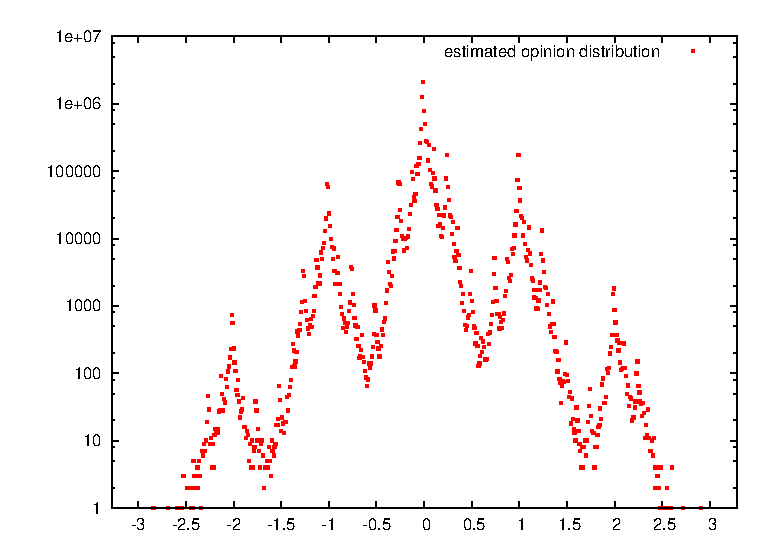
\includegraphics[width=0.75\textwidth]{chapters/03_implementation/opidist_log}
        \caption{Distribution of opinions with $Y$ axis in logarithmic scale.}
        \label{fig:opinion_distribution_log}
      \end{figure}
      The visible peaks are a clear evidence that the majority of messages with opinions are short enough for only several opinions influencing a keyword. Otherwise, the distribution would have had a more smooth, cone-like shape. The perfect cone-like shape would be achieved if posts were consisting of one keyword only with a lot of opinions written on both sides of it. Also, the advantage of positive opinions is more evident using this scale.

    \subsubsection{Problems}

      Checking \emph{opinion sign} is not as easy as determining whether the opinion is positive or negative. The problem is that there exist modifier words that completely change the meaning of word. Examples of words like that include \emph{not} or \emph{don't}.
      
      In order to mitigate this problem and to bias the opinions correctly it was necessary to check for existence of such modifier words in a proximity of opinion words.
      
      Following expressions illustrate the problem: \textquote{\emph{not} \textbf{good},} \textquote{\emph{not} sufficient \textbf{good},} \textquote{\emph{not} at all \textbf{good}.}
      One can clearly see that it is not necessary to check just one word before an opinion. I have decided to cover all three cases like that even though there may be more edge cases. Hence, modifier words were only checked as far as two words from an opinion and were not taken into consideration if there were another opinion or keyword in between them, for example in messages like \textquote{\emph{not} \textbf{bad}, \textbf{good} even,} where not stopping after one opinion have been found would cause the modifier to act on both opinions instead.

  \subsection{Average path length}

    Figure \ref{fig:avg_path} shows changes of average path length calculated for each bucket of data. The general trend shows that the average length of paths in the network has been decreasing. This may be due to the fact that most of the users did not leave the forum and continued to write messages while retaining their connections. Nevertheless the path lengths are much higher, in a range between $3.27$ and $3.55$, than the one calculated for the whole network which was calculated at $2.68$. This is clearly because of the whole network being significantly larger (having more edges), thus having higher probability for connections to exist.
    \begin{figure}[H]
      \centering
      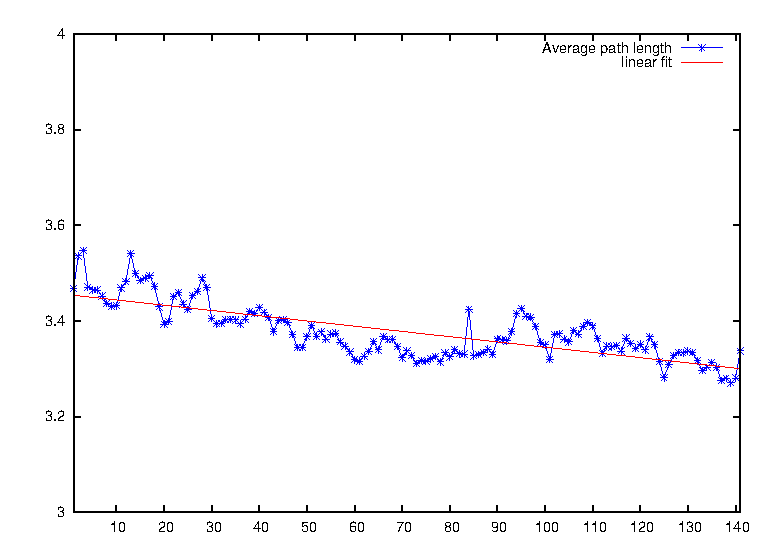
\includegraphics[width=\textwidth]{chapters/03_implementation/avg_path}
      \caption{Changes of average path length over time.}
      \label{fig:avg_path}
    \end{figure}

  \subsection{Collaborative Similarity} \label{sec:cs}
    
    Ming-Sheng Shang \textit{et al.} have proposed a new index called \emph{collaborative similarity}, to quantify the diversity of tastes based on the collaborative selection\cite{Shang2010}. This newly proposed index sounds promising for the data under analysis in this thesis. It may be a good idea to explore and look at the \emph{user-message network} from the other angle and if we can find that the user selection is highly clustered---i.e. not that much diverse---then we will be able to easily identify main groups of users.
    
    \subsubsection{The concept}
    
      Figure \ref{fig:cs_network} illustrates a small bipartite network that consists of six users and eight objects. The degree of user $i$, denoted by $k_i$, is defined as the number of objects connected to $i$. Analogously, the degree of object $\alpha$, denoted by $d_\alpha$, is the number of users connected to $\alpha$. For example, as shown in figure \ref{fig:cs_network}, $k_i = d_\alpha = 3$. The density function, $p(k)$, is the probability that a randomly selected user is of degree $k$, while the cumulative function, $P(k)$, denotes the probability that a randomly selected user is of degree no less than $k$.
      \begin{figure}[h]
        \centering
        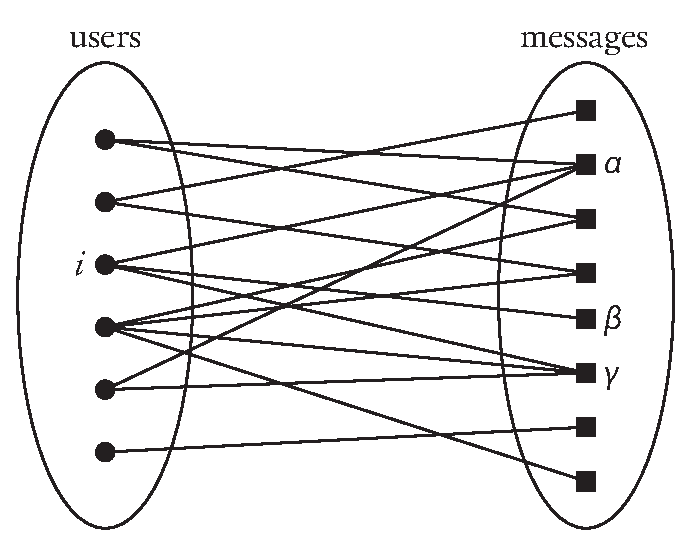
\includegraphics[width=0.6\textwidth]{chapters/03_implementation/cs_network}
        \caption{Small user-message bipartite network.}
        \label{fig:cs_network}
      \end{figure}
      
      The \emph{nearest neighbors’ degree} for user $i$, denoted by $d_{nn}(i)$, is defined as the average degree over all the objects connected to $i$. For example, as shown in figure \ref{fig:cs_network},
      \begin{equation}
        d_{nn}(i) = \frac{d_\alpha + d_\beta + d_\gamma}{3} = \frac{7}{3}\mbox{.}
      \end{equation}

      The degree-dependent nearest neighbors’ degree, $d_{nn}(k)$ is the average nearest neighbors’ degree over all the users of degree $k$, that is,
      \begin{equation}
        d_{nn}(k) = \langle d_{nn}(i) \rangle_{k_i=k}\mbox{.}
      \end{equation}

      Corresponding definitions for objects, say $p(d)$, $P(d)$, $k_{nn}(\alpha)$ and $k_{nn}(d)$, are similar and thus omitted here.
      
      The traditional clustering coefficient\cite{WattsStrogatz1998} cannot be used to quantify the clustering pattern of a bipartite network since it always give a zero value. Lind \textit{et al.}\cite{LindGonzalezHerrmann2005} proposed a variant counting the rectangular relations instead of triadic clustering, which can be applied to general bipartite networks. However, this letter aims at a special class of bipartite networks, and thus we propose a new index to characterise the clustering selections\footnote{Here the term \textquote{clustering} describes the fact that a user's selections are usually very similar to each other, and may belong to a few clusters or communities according to the standard clustering analysis or community detection.} resulted from the collaborative interests of users. A standard measure of object similarity according to the collaborative selection is the \emph{Jaccard similarity}\cite{Jaccard1901}.
      \begin{equation}
        s_{\alpha\beta} = \frac{\Gamma_\alpha \cap \Gamma_\beta}{\Gamma_\alpha \cup \Gamma_\beta}\mbox{,}
      \end{equation}
      where $\Gamma_\alpha$ and $\Gamma_\beta$ are the sets of neighbouring nodes of $\alpha$ and $\beta$, respectively. Obviously, $s_{\alpha\beta} = s_{\beta\alpha}$ and $0 \leq s_{\alpha\beta} \leq 1$ for any $\alpha$ and $\beta$. For example, as shown in figure \ref{fig:cs_network}, $s_{\alpha\beta} = s{\beta\gamma} = \sfrac{1}{3}$ and ${\alpha\gamma} = \sfrac{1}{2}$. The collaborative similarity of user $i$ is then defined as the average similarity between $i$'s selected objects:
      \begin{equation}
        C_u(i) = \frac{1}{k_i(k_i-1)} \sum_{\alpha\neq\beta} s_{\alpha\beta}\mbox{,}
      \end{equation}
      where $\alpha$ and $\beta$ run over all $i$'s neighbouring objects. For example, as shown in figure \ref{fig:cs_network}, the collaborative similarity of user $i$ is $C_u(i) = \sfrac{7}{18}$. According to the definition, a user whose collections are very similar to each other will have high collaborative similarity. For example, a user who only watches science fiction movies is probably of higher collaborative similarity than the one who has very diverse interests of movies. The user collaborative similarity of the whole network is defined as
      \begin{equation}
        C_u = \frac{1}{N^\prime} \sum_{i} C_u(i)\mbox{,}
      \end{equation}
      where $i$ runs over all users with degrees larger than $1$ and $N^\prime$ denotes the number of these users. The degree-dependent collaborative similarity, $C_u(k)$, is defined as the average collaborative similarity over all the $k$-degree users. Corresponding definitions for objects are as following:
      \begin{equation}
        C_o(\alpha) = \frac{1}{d_\alpha(d_\alpha-1)} \sum_{i\neq j} s_{ij}\mbox{,}
      \end{equation}
      where $s_{ij} = \left| \frac{\Gamma_i \cap \Gamma_j}{\Gamma_i \cup \Gamma_j} \right|$ is the Jaccard similarity between users $i$ and $j$ and:
      \begin{equation}
        C_o = \frac{1}{M^\prime} \sum_\alpha C_o(\alpha)\mbox{,}
      \end{equation}
      where $M^\prime$ denotes the number of objects with degrees larger than $1$. $C_o(d)$ is the average collaborative similarity over all the $d$-degree objects.

    \subsubsection{Results}
    
      \begin{table}[h]
        \begin{tabularx}{\textwidth}{|C{1.1}|C{0.95}|C{0.95}|C{1}|C{1}|C{1}|C{1}|C{1}|C{1}|C{1}|} \hline
          \rowcolor[gray]{0.75} \textbf{Bucket} & $N$ & $M$ & $E$ & $\langle k \rangle$ & $\langle d \rangle$ & $C_u$ & $\bar s_m$ & $C_m$ & $\bar s_u$ \\\hline
$1$ & $193$ & $2616$ & $29560$ & $78.02$ & $5.76$ & $0.1608$ & $0.1046$ & $0.1278$ & $0.1453$ \\\hline
$11$ & $417$ & $3647$ & $55201$ & $68.54$ & $7.84$ & $0.1376$ & $0.0955$ & $0.1182$ & $0.1148$ \\\hline
$21$ & $609$ & $3787$ & $73964$ & $62.79$ & $10.10$ & $0.1253$ & $0.0936$ & $0.1167$ & $0.1028$ \\\hline
$31$ & $718$ & $4027$ & $89545$ & $63.74$ & $11.37$ & $0.1235$ & $0.0926$ & $0.1166$ & $0.0986$ \\\hline
$41$ & $942$ & $4247$ & $93741$ & $55.60$ & $12.33$ & $0.1070$ & $0.0860$ & $0.1047$ & $0.0857$ \\\hline
$51$ & $1318$ & $4622$ & $118121$ & $51.71$ & $14.75$ & $0.0975$ & $0.0812$ & $0.0995$ & $0.0768$ \\\hline
$61$ & $1966$ & $5232$ & $191560$ & $54.71$ & $20.56$ & $0.0988$ & $0.0849$ & $0.1033$ & $0.0747$ \\\hline
$71$ & $1701$ & $5095$ & $89352$ & $52.53$ & $17.54$ & $0.0975$ & $0.0800$ & $0.0996$ & $0.0741$ \\\hline
$81$ & $1905$ & $5090$ & $91795$ & $48.19$ & $18.03$ & $0.0932$ & $0.0787$ & $0.0985$ & $0.0711$ \\\hline
$91$ & $1680$ & $4774$ & $77094$ & $45.89$ & $16.15$ & $0.0900$ & $0.0775$ & $0.0935$ & $0.0736$ \\\hline
$101$ & $1817$ & $5544$ & $105478$ & $58.05$ & $19.03$ & $0.1096$ & $0.0867$ & $0.1103$ & $0.0799$ \\\hline
$111$ & $1743$ & $4989$ & $81130$ & $46.55$ & $16.26$ & $0.0918$ & $0.0777$ & $0.0961$ & $0.0716$ \\\hline
$121$ & $1706$ & $4900$ & $81357$ & $47.69$ & $16.60$ & $0.0968$ & $0.0784$ & $0.1000$ & $0.0755$ \\\hline
$131$ & $1994$ & $5562$ & $104444$ & $52.38$ & $18.78$ & $0.0986$ & $0.0796$ & $0.1011$ & $0.0732$ \\\hline
$141$ & $2080$ & $5250$ & $94994$ & $45.67$ & $18.09$ & $0.0915$ & $0.0757$ & $0.0962$ & $0.0712$ \\\hline        \end{tabularx}
        \caption{The basic properties of every 10th data bucket.}
        \label{tab:cs_properties}
      \end{table}

      Table \ref{tab:cs_properties} summarises basic statistics of selected data buckets. $N$, $M$ and $E$ denote the number of users, messages and edges connecting them, respectively. $\langle k \rangle$ and $\langle d \rangle$ are the average user degree and average message degree. $C_u$ and $C_m$ are the average collaborative similarity for users and messages, and for comparison, $\bar s_m$ and $\bar s_u$ are the average similarities over all message pairs and over all user pairs, respectively. The user selection is considered to be poorly clustered (i.e., more diverse) because the condition for that is $C_u \gg \bar s_m$ whereas $C_u$ is the same order of magnitude as $\bar s_m$. Unfortunately, this basically means that it will not be easy to identify groups of users that may have formed in this message board and I had to abandon this somewhat interesting index. Figure \ref{fig:cs_cusm} show the way $C_u$ and $\bar s_m$ were changing over time. In no bucket, $C_u$ was much greater than $\bar s_m$ and even in bucket 84 they were pretty close to each other: $0.0746$ vs $0.0683$ respectively.
      This does not however disqualify that method completely. The results only mean that it will not be easy to find any anomalies. There are $52605$ users in the database so I could just run over a $C_u(i)$ of every user and look for suspicious changes. However strenuous it sounds, it may be worth it. What we are looking for are users whose $C_u(i)$ is significantly different than it was before, incidating possible \emph{marketing campaign}.
      \begin{figure}[H]
        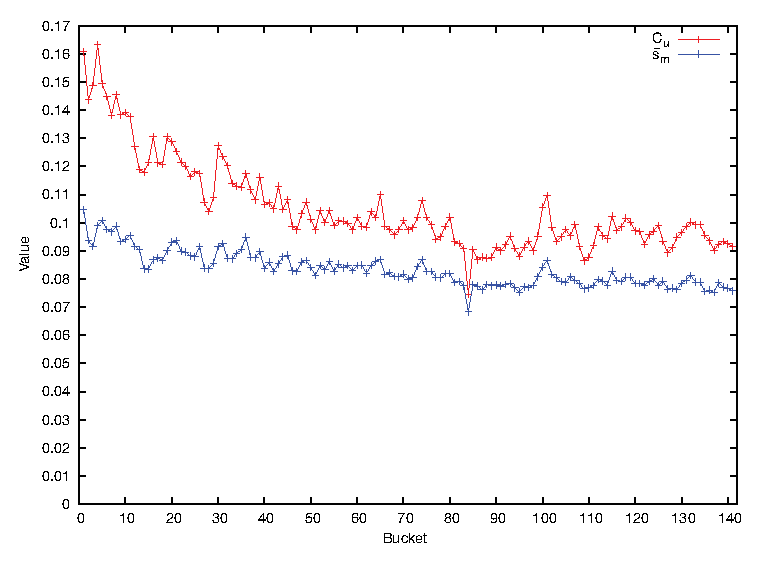
\includegraphics[width=0.9\textwidth]{chapters/03_implementation/C_us_m}
        \caption{Changes of $C_u$ and $\bar s_m$ over time.}
        \label{fig:cs_cusm}
      \end{figure}

      Figure \ref{fig:cs_dist_full} represents distribution of $C_u(i)$ across all users. Where $C_u(i)$ was in a range $[0, 1]$ it was stretched to $[0, 100]$ to create $101$ distinct buckets so that the distribution may have been calculated. Large number of nodes in \textquote{$0$} bucket constitutes with rather big amount of users with the degree less than or equal to $1$, where $C_u(i)$ is calculated as $0$ for such degree. Figure \ref{fig:cs_dist_tail} shows the tail of the distribution from figure \ref{fig:cs_dist_full} as it is not visible due to the scale used.
      \begin{figure}[H]
        \centering
        \begin{subfigure}[b]{0.49\textwidth}
          \centering
          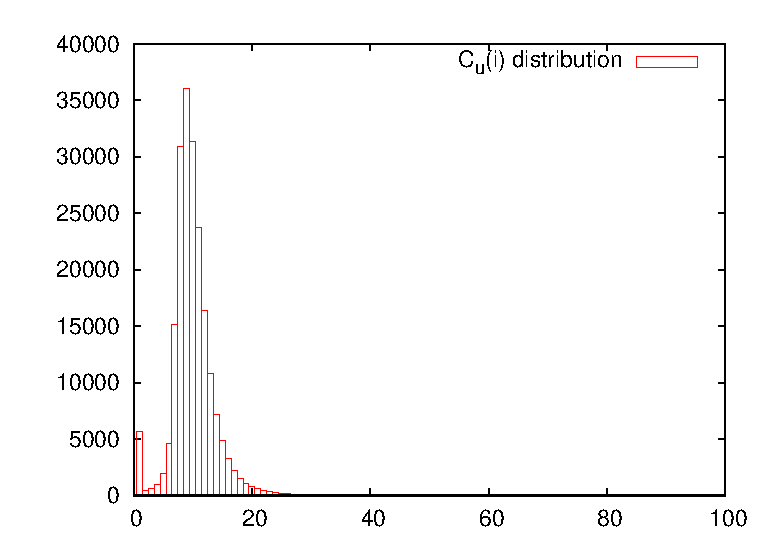
\includegraphics[width=\textwidth]{chapters/03_implementation/cs_dist}
          \caption{Full scale.}
          \label{fig:cs_dist_full}
        \end{subfigure}
        \begin{subfigure}[b]{0.49\textwidth}
          \centering
          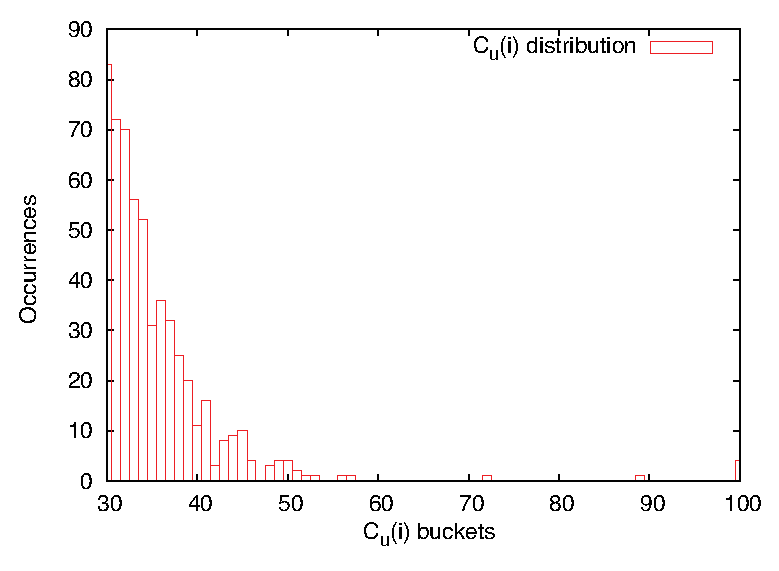
\includegraphics[width=\textwidth]{chapters/03_implementation/cs_dist_tail}
          \caption{The tail.}
          \label{fig:cs_dist_tail}
        \end{subfigure}
        \caption{Distribution of $C_u(i)$ across all users.}
      \end{figure}
      
      Figure \ref{fig:cu_12195} shows changes of $C_u(i)$ for user $i=12195$. One can clearly tell that the collaborative similarity for that user suddenly peaks three times as it was before. The next step would involve looking at the individual messages posted by that user during the time the peak occurred (bucket number 107).
      \begin{figure}[h!]
        \centering
        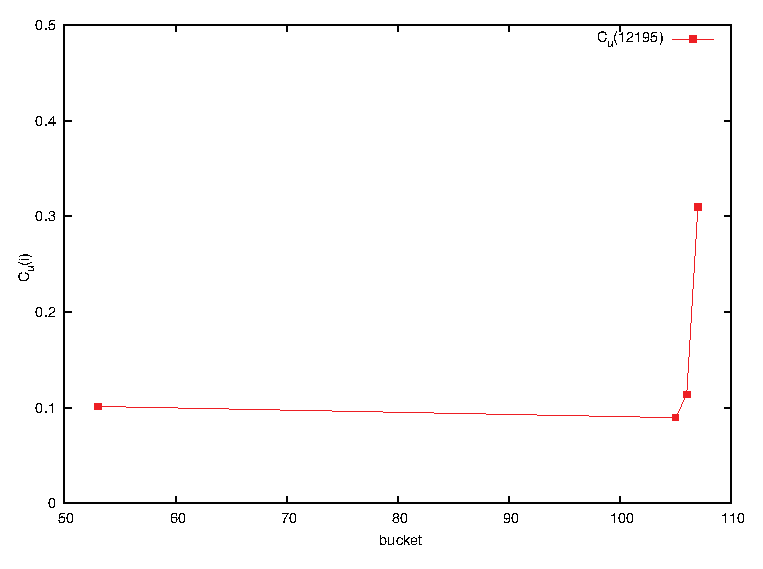
\includegraphics[width=0.8\textwidth]{chapters/03_implementation/u12195}
        \caption{Changes of $C_u(i)$ for $i=12195$.}
        \label{fig:cu_12195}
      \end{figure}
      
      After reading the posts, it looks like one of the forum users started a \textquote{headphone brand elimination game!} topic on July 27, 2009 that was active until August 25, 2009 (buckets 106-107). The rules of the game were simple:
      \begin{enumerate}
        \item The topic started with brand names written down along with initial 10 health points.
        \item Users were supposed to post a message containing one brand they want to hurt or heal, adding or removing one health point respectively.
        \item Health points did not stack above 20.
        \item A brand would lose---thus removed from the list effectively---once it was left with 0 health points.
        \item Once four brands were left on the battlefield, their health was restored according to some other rules and the battle followed until one winner has left standing.
      \end{enumerate}
      The battle struggled between brands \emph{Sennheiser} and \emph{STAX} for a longer period, with the former eventually winning 20-0. I think that the analysis of this topic alone would bring some interesting results. The only problem is that, because of this topic, I had to completely skip the results for buckets 106 and 107 due to the fact that the results would be distorted.
      
    \subsubsection{$C_u(i)$ fluctuation patterns found} \label{sec:cs_fluctuations}
    
      Figure \ref{fig:cs_fluctuations} shows various types of patters of $C_u(i)$ fluctuations that seem to repeat throughout individual users. I will not try to interpret these as it would require further, thorough examination which I did not perform due to time constraints.
      
      \begin{figure}[H]
        \centering
        \begin{subfigure}[b]{0.32\textwidth}
          \centering
          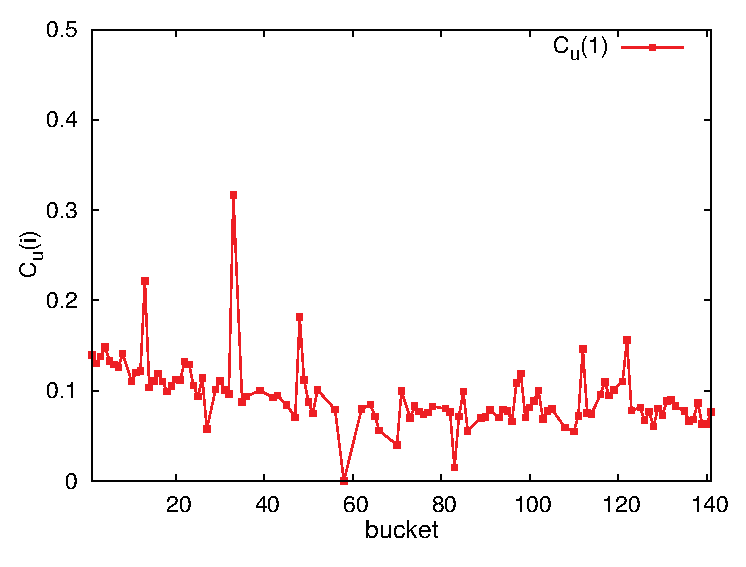
\includegraphics[width=\textwidth]{chapters/03_implementation/u1}
        \end{subfigure}
        \begin{subfigure}[b]{0.32\textwidth}
          \centering
          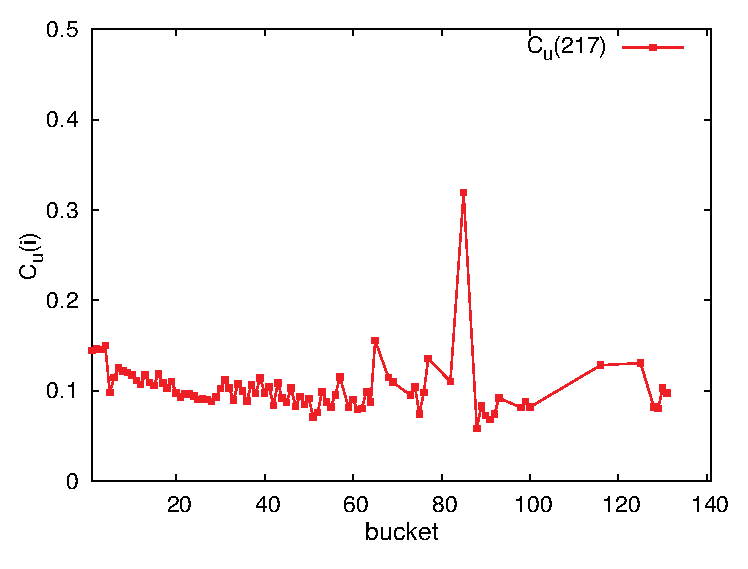
\includegraphics[width=\textwidth]{chapters/03_implementation/u217}
        \end{subfigure}
        \begin{subfigure}[b]{0.32\textwidth}
          \centering
          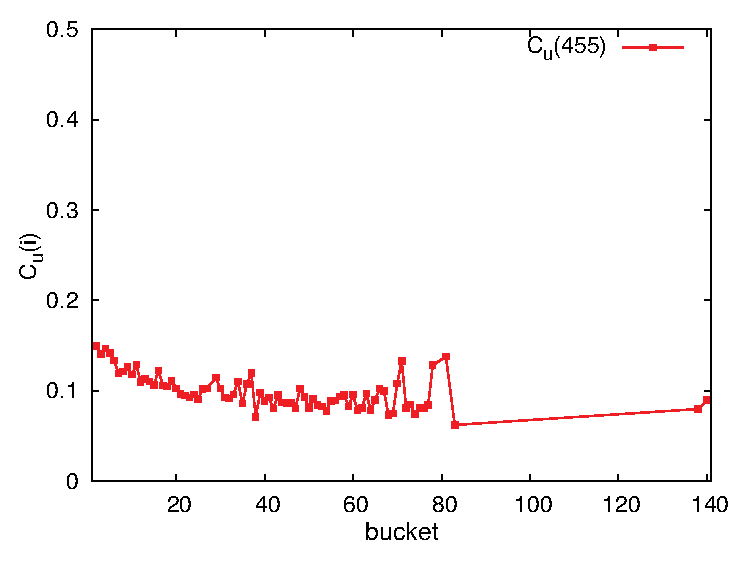
\includegraphics[width=\textwidth]{chapters/03_implementation/u455}
        \end{subfigure}
        \begin{subfigure}[b]{0.32\textwidth}
          \centering
          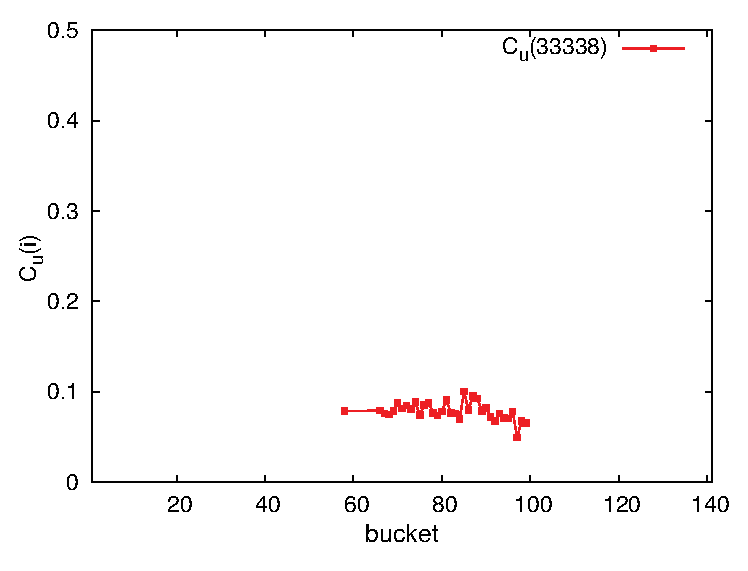
\includegraphics[width=\textwidth]{chapters/03_implementation/u33338}
        \end{subfigure}
        \begin{subfigure}[b]{0.32\textwidth}
          \centering
          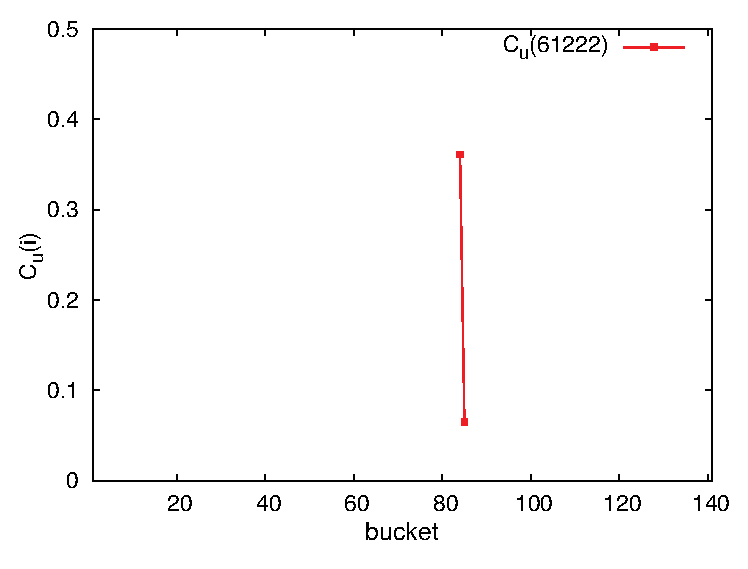
\includegraphics[width=\textwidth]{chapters/03_implementation/u61222}
        \end{subfigure}
        \begin{subfigure}[b]{0.32\textwidth}
          \centering
          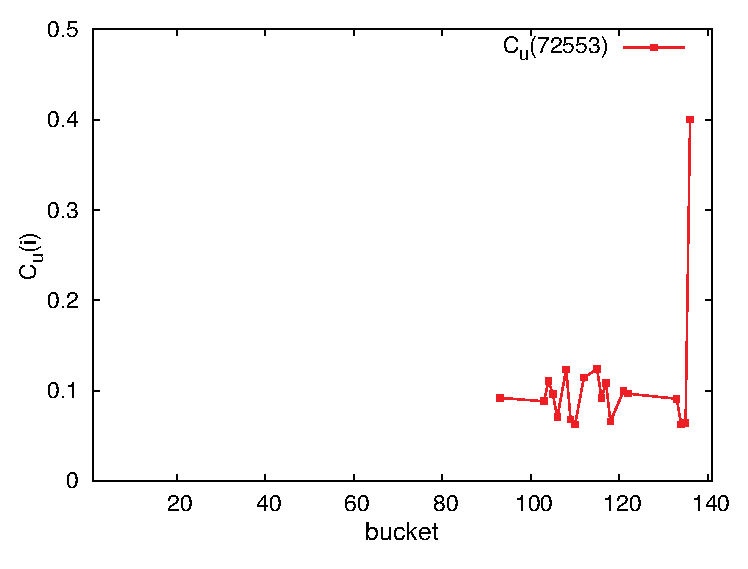
\includegraphics[width=\textwidth]{chapters/03_implementation/u72553}
        \end{subfigure}
        \begin{subfigure}[b]{0.32\textwidth}
          \centering
          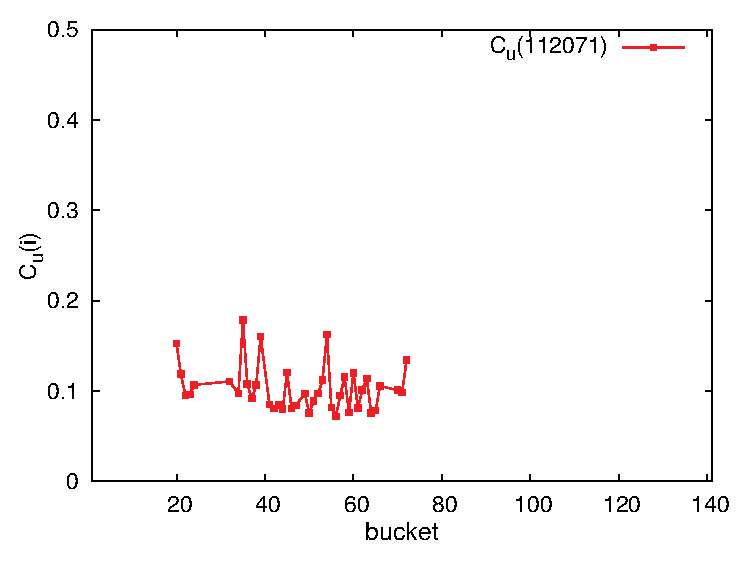
\includegraphics[width=\textwidth]{chapters/03_implementation/u112071}
        \end{subfigure}
        \begin{subfigure}[b]{0.32\textwidth}
          \centering
          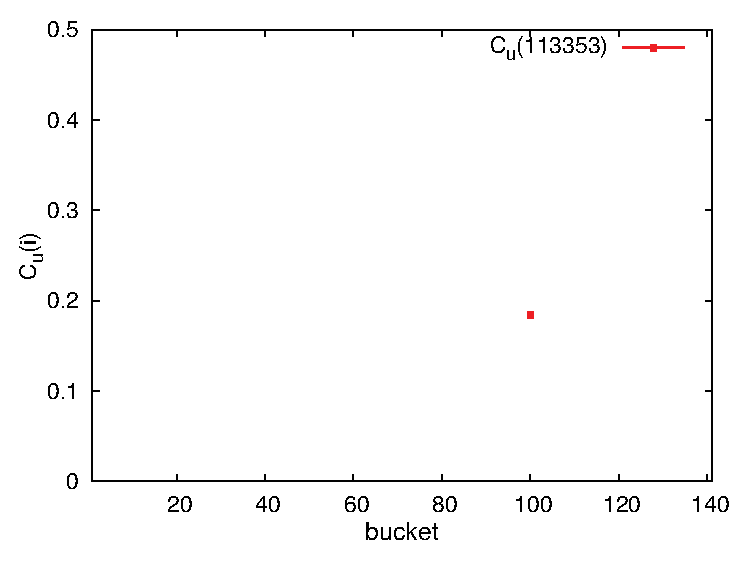
\includegraphics[width=\textwidth]{chapters/03_implementation/u113353}
        \end{subfigure}
        \begin{subfigure}[b]{0.32\textwidth}
          \centering
          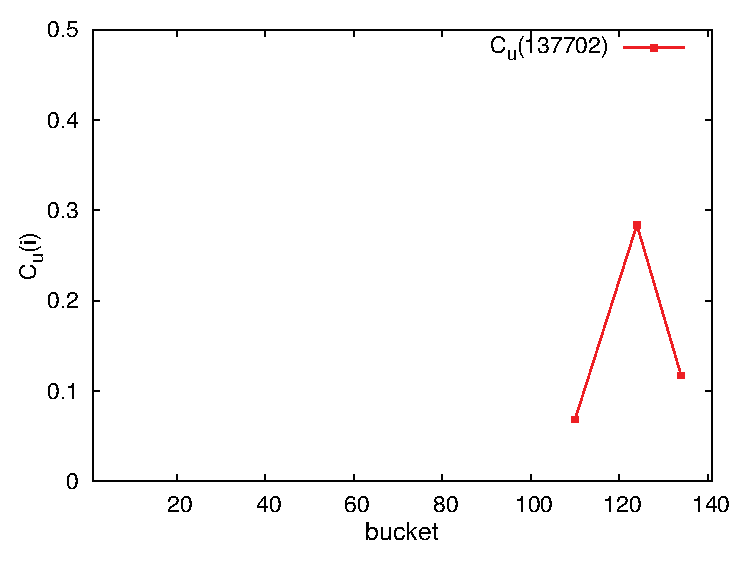
\includegraphics[width=\textwidth]{chapters/03_implementation/u137702}
        \end{subfigure}
        \caption{Patterns of $C_u(i)$ fluctuations.}
        \label{fig:cs_fluctuations}
      \end{figure}

  \subsection{Motifs}
  
    \subsubsection{Introduction}
      
      One of the methods that I was sure will bring up some groups of users was the motif discovery within the network. It was found that real world network often feature recurrent sub-graphs or patterns. \emph{Motifs} are sub-graphs that repeat themselves in the network or even in networks of the same type. Indeed, motifs are of notable importance largely because they may reflect functional properties. They have recently gathered much attention as a useful concept to uncover structural design principles of complex networks\cite{MasoudiSchreiberKashani2012}.
      
      Network motifs were at first defined systematically in \emph{Escherichia coli}, where they were detected as patterns that occurred in the transcription network much more often than would be expected in random networks\cite{MiloAlon2002}. The exact same motifs have been later found in other organisms, ranging from other bacteria\cite{ManganZaslaverAlon2003,Eichenberger2004} and yeast\cite{MiloAlon2002, Lee2002}, to plants\cite{Saddic2006} and animals\cite{Boyer2005}. Motif discovery have been the most successful in biological networks, most likely because they were the most studied at the time---especially the transctiption networks. I will not explain many details about the motifs, because this is a complicated matter and already has been discussed and reviewed thoroughly\cite{Alon2007}.
      
    \subsubsection{Motif discovery}
    
      Although network motifs may provide a deep insight into the network's functional abilities, their detection is computationally challenging. Because of that, I have decided to only concentrate on the most basic, triangle motifs, that I have discovered using not very sophisticated algorithm conjoining two users sharing similar opinions about particular brands, hoping that this approach will lead to some interesting opportunities. This also allowed me to map the bipartite network I was working on so far to a regular network built on a set of users exchanging opinions only. Because I have already joined users with brands they were discussing based on the opinion being positive, negative or neutral, the only step required to obtain these triangles was to link users with matching opinions. Data required for motif discovery has been obtained in section \ref{sec:opinion_estimation}.
      
      First, the algorithm builds a bipartite network with users and opinions about the brands. Edges (solid lines) represent the opinion the user has about the product. It is not possible to have more than one edge between the nodes, because all opinions about the brand users may have are averaged and only this average number is taken into account during network creation. When the network is ready, algorithm finds user nodes having edges to the same brand nodes and links them together (dashed lines). The final step involves deletion of initial edges along with brand nodes resulting in non-bipartite network consisting of user nodes only. Figure \ref{fig:motifs_alg} illustrates steps taken by the algorithm.
      \begin{figure}[h]
        \centering
        \begin{subfigure}[b]{0.3\textwidth}
          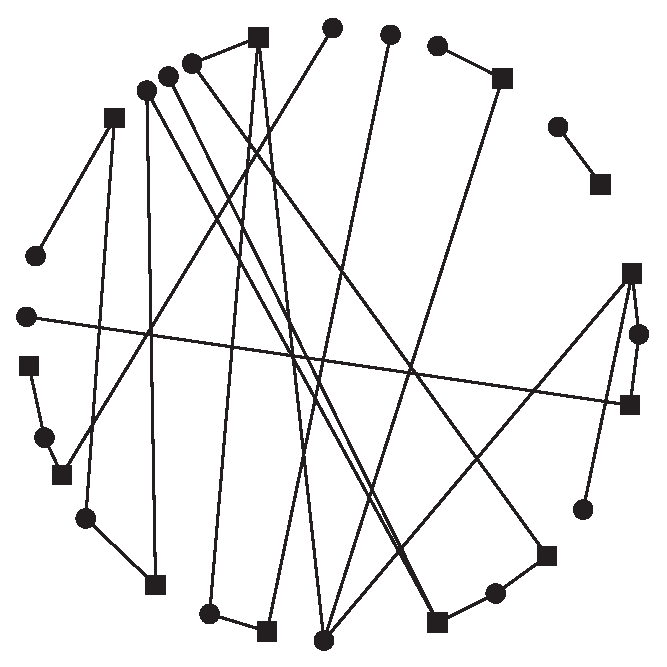
\includegraphics[width=\textwidth]{chapters/03_implementation/cs_motif_1}
          \caption{Step 1.}
          \label{fig:motifs_alg_1}
        \end{subfigure}
        \quad
        \begin{subfigure}[b]{0.3\textwidth}
          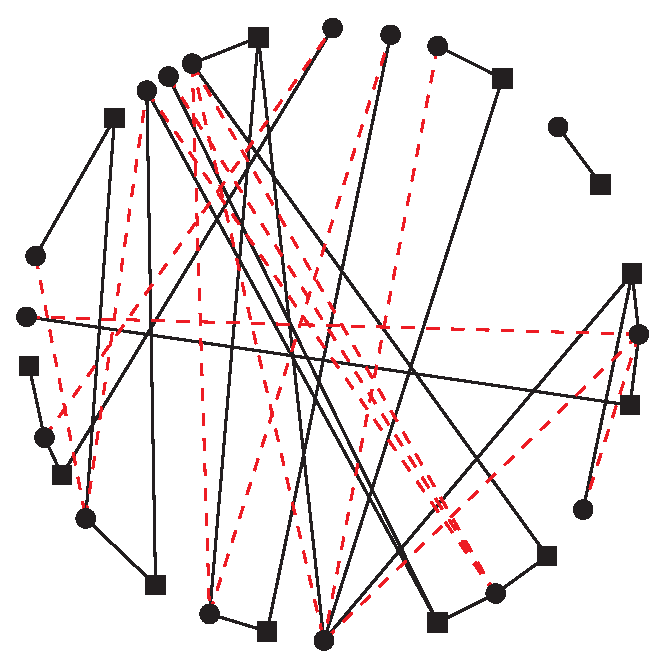
\includegraphics[width=\textwidth]{chapters/03_implementation/cs_motif_2}
          \caption{Step 2.}
          \label{fig:motifs_alg_2}
        \end{subfigure}
        \quad
        \begin{subfigure}[b]{0.3\textwidth}
          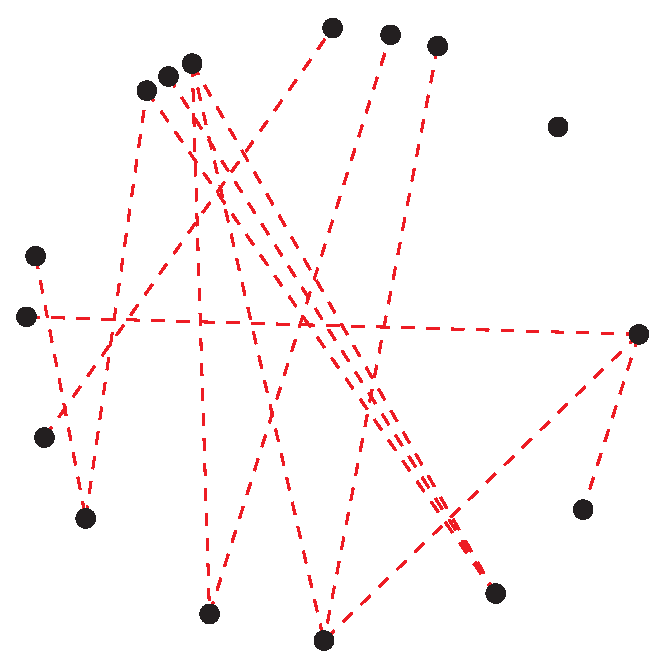
\includegraphics[width=\textwidth]{chapters/03_implementation/cs_motif_3}
          \caption{Step 3.}
          \label{fig:motifs_alg_3}
        \end{subfigure}
        \caption{Algorithms steps.}
        \label{fig:motifs_alg}
      \end{figure}
      Graphs in figures \ref{fig:motifs_alg_1} and \ref{fig:motifs_alg_2} are bipartite and in figure \ref{fig:motifs_alg_3} the graph is a non-bipartite graph projected from bipartite network. Circled nodes represent users and squared nodes represent words (brand names). Solid edges show which words were used by which users and dashed edges serve as an opinion shared between two users about a brand.
      
    \subsubsection{Substructures derived from motif analysis}
      
      Figure \ref{fig:motif_network} shows a fragment of network created with the above method from bucket 106 which was excluded before in section \ref{sec:cs_results}. The network is a multigraph with nodes representing the users and edges representing an opinion about a brand shared between two users.
      \begin{figure}[b!]
        \centering
        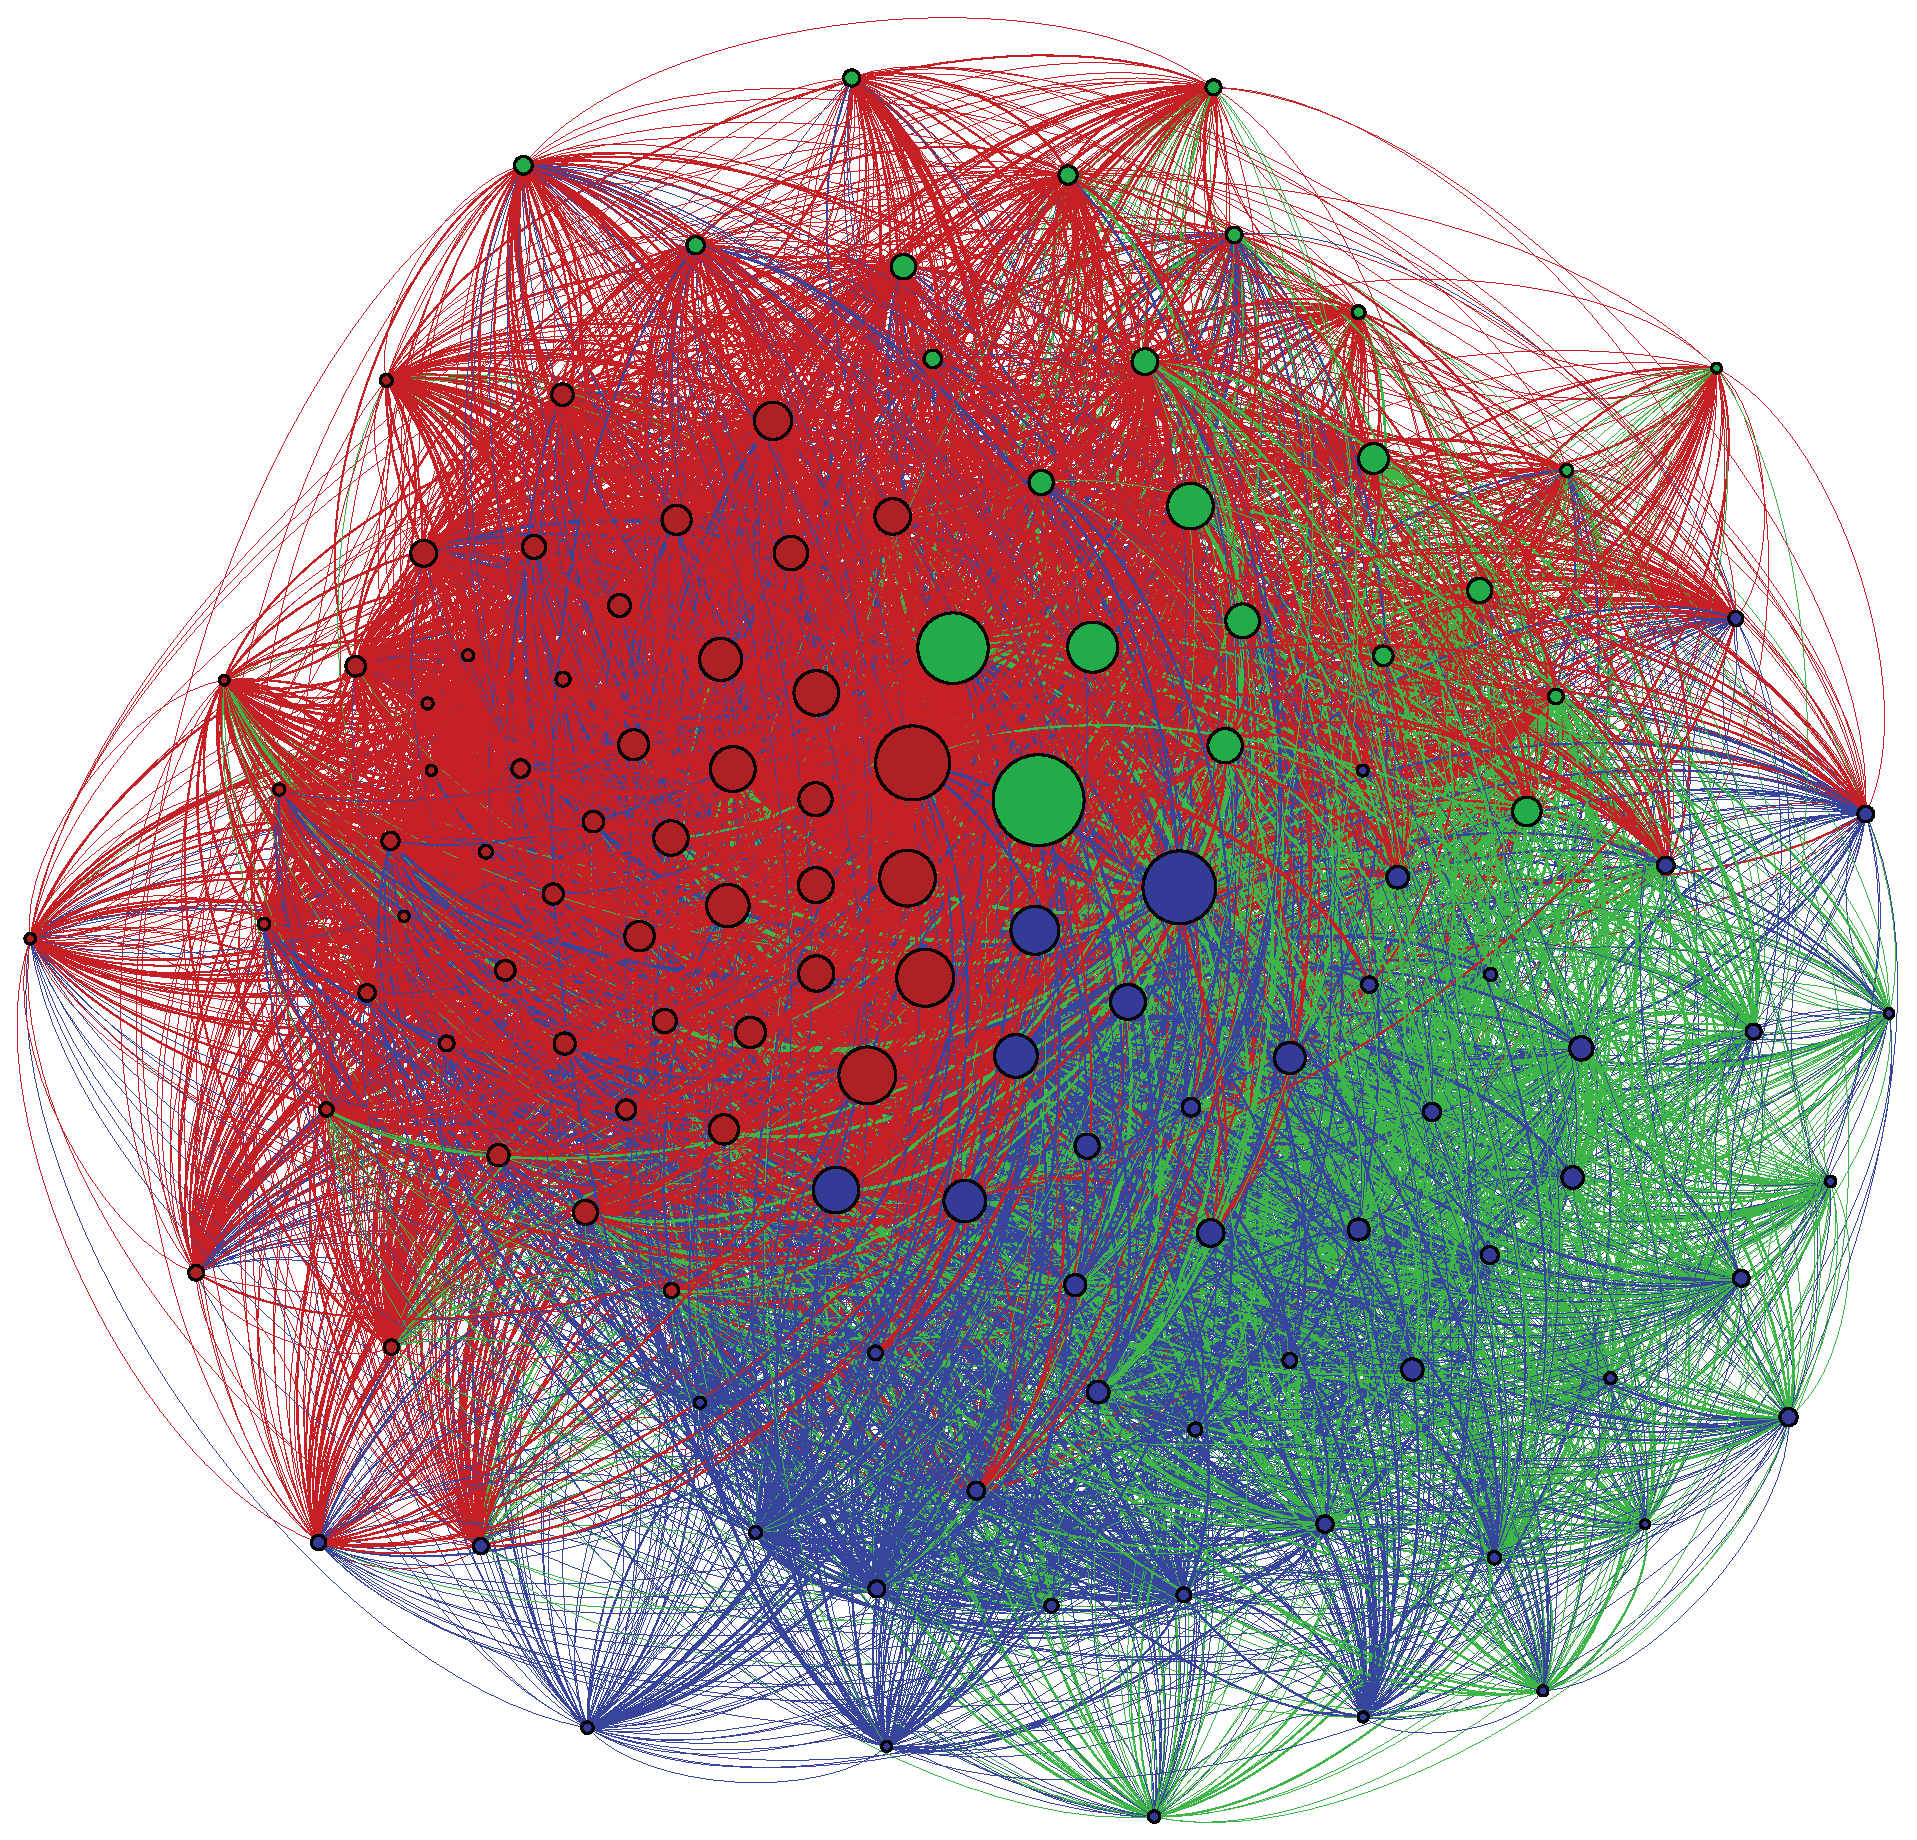
\includegraphics[width=0.66\textwidth]{chapters/03_implementation/motif_network}
        \caption{Network obtained with motif discovery.}
        \label{fig:motif_network}
      \end{figure}
      
      The network was constructed using opinions about 10 brands presented in table \ref{tab:motif_brands} ordered by the number of times they were used in that bucket. Even though \emph{Stax} won the game mentioned in section \ref{sec:cs_results} it was not discussed between the users in an essential manner. The number of opinions about that brand was so low that it did not matter in the whole network. The size of each node was determined from it's betweenness centrality to stress the importance of certain nodes in this network despite the fact that degrees are fairly equal and distributed uniformly in a range $[100:216]$.
      
      Three brands were discussed in a particularly frequent manner between the users, thus the network consisted mostly of opinions about them. Hence, the classes of users presented in figure \ref{fig:motif_network} are made of three brands discussed the most: \emph{Grado}, \emph{Sennheiser} and \emph{Denon}. Grado was discussed the most (see table \ref{tab:motif_brands}), but only $18.93\%$ of shared opinions in the network are about this brand. This means that the opinions about Grado (green edges) are inconsistent, so users sharing opinion about Sennheiser or Denon does not share opinion about Grado in general. 
      \begin{table}[H]
        \centering
        \begin{tabularx}{0.6\textwidth}{|L{0.6}|L{1.2}|L{1.2}|} \hline
          \rowcolor[gray]{0.8} \textbf{Position} & \textbf{Brand} & \textbf{Times used} \\\hline
          1 & Grado & $1,948$ \\\hline
          2 & Sennheiser & $1,408$ \\\hline
          3 & Denon & $881$ \\\hline
          4 & AKG & $804$ \\\hline
          5 & Stax & $560$ \\\hline
          6 & Beyerdynamic & $423$ \\\hline
          7 & Sony & $411$ \\\hline
          8 & Yamaha & $364$ \\\hline
          9 & Bose & $212$ \\\hline
          10 & Panasonic & $132$ \\\hline
        \end{tabularx}
        \caption{Brands used to create network shown in figure \ref{fig:motif_network}.}
        \label{tab:motif_brands}
      \end{table}
      While Denon was the least discussed from \textquote{the great three} it certainly indicates that users' opinions are reciprocal with over half ($53.56\%$) of the network edges (red coloured) joining users. Opinions about Sennheiser (blue links) form the other $27.51\%$ of the network. Vertices were coloured with the colour of edges that were linked to that vertex the most.
      
      Particularly interesting is the case of users that either do not discuss some brands (more likely) or have no common opinions about that brand (much less likely) with other users. This means that a substructure may exist where users are focused on several brands only and do not discuss others at all. The conclusions here might be too far-reaching, but this idea might be interesting to tackle.
      
      The average path length is $1.143$ which is extremely short and shows how efficient the network is. The average clustering coefficient for this network was calculated as $0.891$. The graph is nearly complete with a density being equal to $0.857$ meaning that almost every user in this network share a similar opinion with another one. The network was meant to be maximally dense, so I would say that the missing $0.143$ density constitute a contradictory opinions.